\chapter{\uppercase{Reactor Neutrinos}}

Nuclear reactors are a pure source of electron antineutrinos, $\bar{\nu_e}$, as a result of the fission of isotopes used in the reactor fuel. The first neutrino was discovered using the nuclear reactor at the Savannah River Plant, and reactor sites continue to be popular homes for neutrino detectors. 
In order to perform precision reactor neutrino studies it is important to understand the reactor neutrino flux and spectrum.

\section{Production of Reactor Neutrinos}

Nuclear reactors are powered by the fission of uranium and plutonium isotopes in their cores. 
Specifically, in a power reactor, 99.9\% of the power comes from the fission of $^{235}$U, $^{239}$Pu, $^{241}$Pu, and $^{238}$U isotopes. 
The reaction begins with a neutron colliding with a nucleus of one of the isotopes. 
This causes the nucleus to split into two fragments, usually of unequal mass, creating an unstable system.
In order to reach stability neutrons have to transform into protons, a process accomplished through $\beta$ decay, see Figure~\ref{fig:nucchart}.
Each beta decay produces an electron and corresponding electron antineutrino. 
In general a nuclear reactor will produce $\sim 6 \times 10^{20} \bar{\nu_e}$ per GW of thermal energy power \cite{HayesVogel}.

\begin{figure}[h]
	\centering
	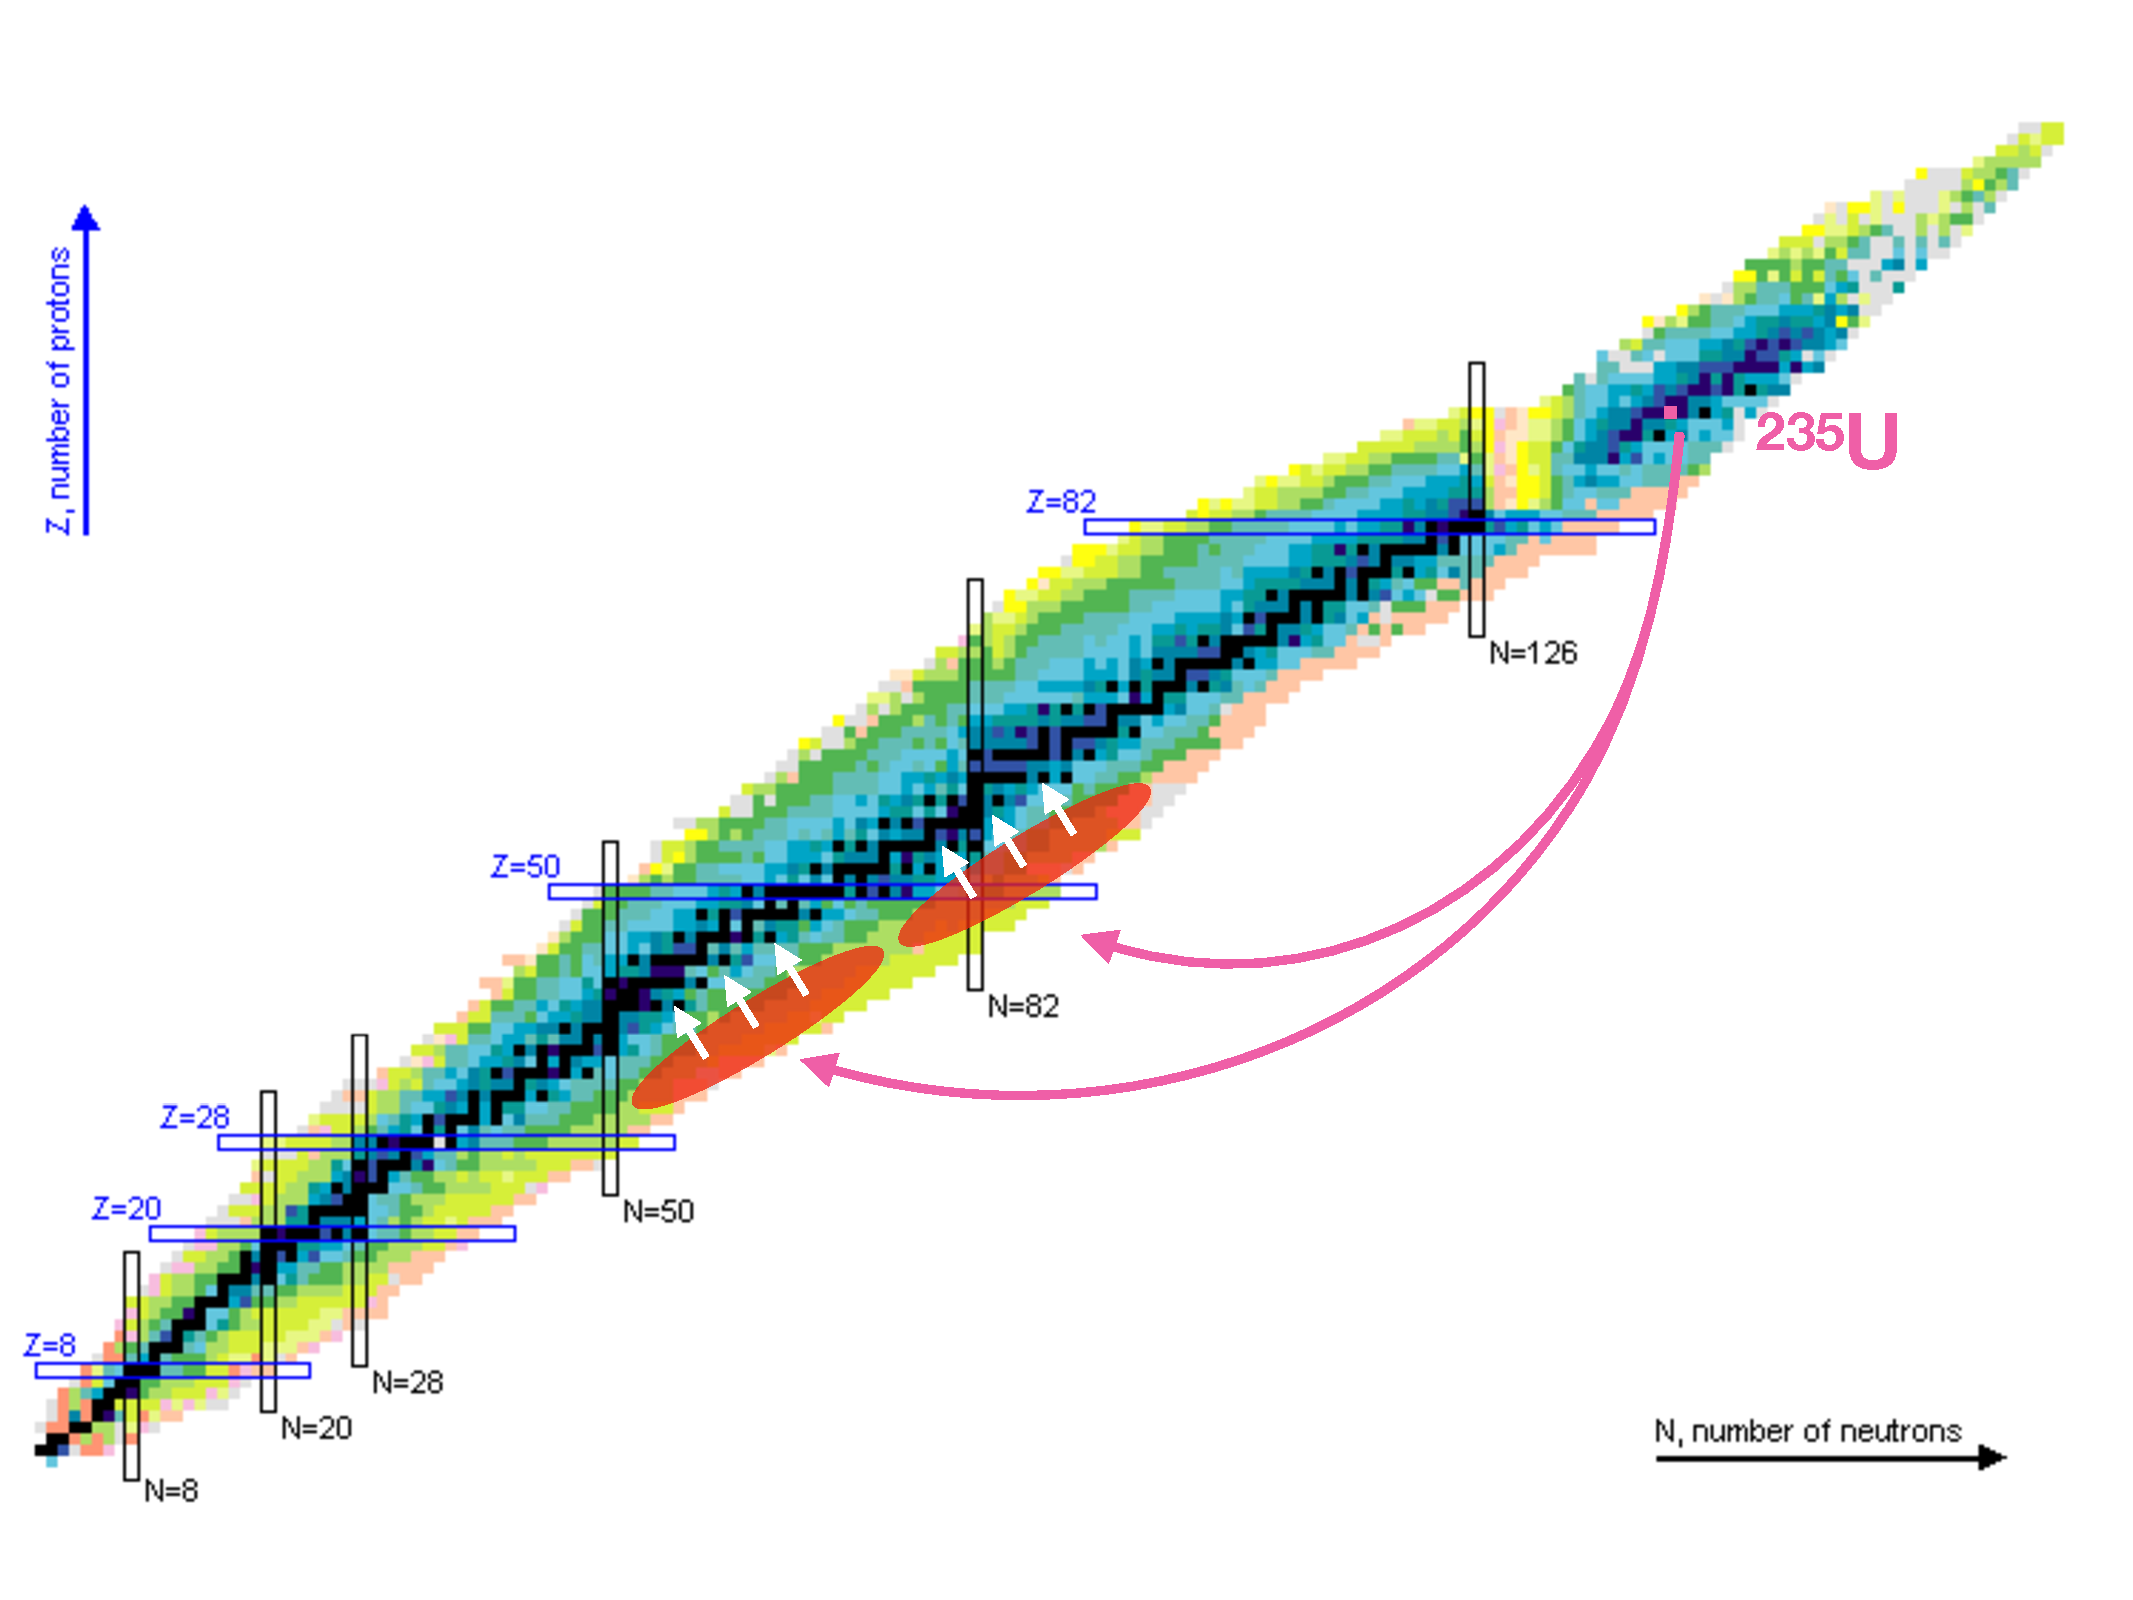
\includegraphics[width=0.7\linewidth]{tex/3-reactorneutrinos-images/NuclideChart_U235}
	\caption[Fission of $^{235}$U.]{A schematic of the fission of $^{235}$U \cite{NucChart}. After collision with a neutron $^{235}$U will split into two unstable nuclei (pink arrows) which will then $\beta$ decay (white arrows) until stable.}
	\label{fig:nucchart}
\end{figure}


\section{Measuring the Reactor Antineutrino Flux and Spectrum}

The total $\bar{\nu_{e}}$ flux, $S(E_\nu)$, produced by a nuclear reactor can be expressed as the sum over the spectra of the dominant fissioning isotopes,
\begin{equation}
	S(E_\nu) = \frac{W_{th}}{\sum_{i}(f_i/F)e_i}\sum_{i}\frac{f_i}{F}\left(\frac{dN_i}{dE_\nu}\right) ,
\end{equation}
where $f_i/F$ is the fission fraction for each given isotope $i$, $W_{th}$ is the reactor thermal energy, $e_i$ is the 
average energy released per fission by each isotope, and $dN_i/dE_\nu$ is the cumulative $\bar{\nu_e}$ spectrum of $i$ normalized per fission.

There are two methods used to determine the $\bar{\nu_e}$ spectrum, \textit{ab initio} summation and electron spectrum conversion.
In the \textit{ab initio} approach the spectrum is determined by summing the contributions of all $\beta$-decay branches of all fission fragments,
\begin{equation}
	\frac{dN_i}{dE_{\bar{\nu}}} =  \sum_{n}Y_n(Z,A,t)\sum_{n,i}b_{n,i}(E^i_0)P_{\bar{\nu}}(E_{\bar{\nu}},E^i_0,Z) ,
\end{equation}
where $Y_n(Z,A,t)$ is the number of $\beta$ decays of the fission fragment $Z, A$ at time $t$, $b_{n,i}(E^i_0)$ are the branching ratios with endpoint energies $E^i_0$, and $P_{\bar{\nu}}(E_{\bar{\nu}},E^i_0,Z)$ is the normalized $\bar{\nu_e}$ spectrum for the branch $n, i$.
This method relies on nuclear databases, such as the Evaluated Nuclear Data File (ENDF) and Joint Evaluated Fission and Fusion (JEFF) databases, for information about the branching ratios and decay energies. 
The antineutrino spectrum for the four main reactor isotopes calculated using \textit{ab initio} summation was done in Ref.~\cite{HayesVogel} and the result can be seen in Figure~\ref{fig:spectrum}. 

Though seemingly straightforward, this approach comes with some caveats.
The shear number of daughter isotopes ($>$1000) and individual $\beta$ decay branches ($>$6000) make the summation non-trivial.
This, along with the fact that not all branching ratios are known, and that the fission yields have been determined by several different database groups but don't always agree and have large uncertainties bring into question the validity of using only this method. 

\begin{figure}[t]
	\centering
	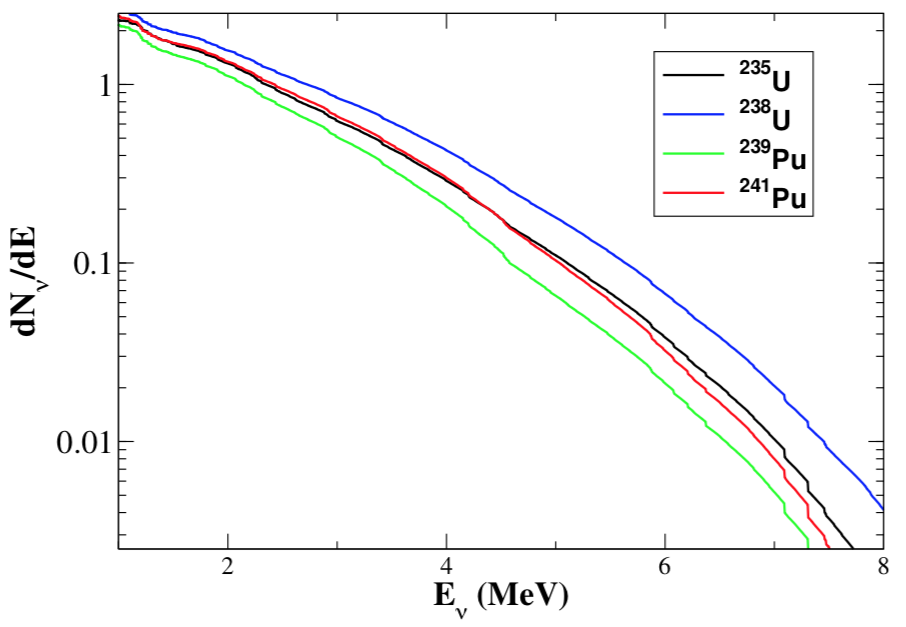
\includegraphics[width=0.65\linewidth]{tex/3-reactorneutrinos-images/Spectrum}
	\caption[The $\bar{\nu_e}$ spectrum.]{The $\bar{\nu_e}$ spectrum predicted by the summation method using the JEFF-3.1.1 database fission fragment yields and the ENDF/B-VII.1 decay library \cite{HayesVogel}.}
	\label{fig:spectrum}
\end{figure}

The other approach to determine the $\bar{\nu_{e}}$ spectrum, the conversion method, relies on converting a measured electron spectrum into an antineutrino spectrum. 
This involves fitting an experimentally defined total beta spectrum with individual beta spectrum  according to their amplitudes, $a_i$, 
\begin{equation}
	\frac{dN_i}{dE_e} = \sum_{i}a_iP(E,E^i_0,Z)
\end{equation}
The conversion to the antineutrino spectrum is then accomplished by replacing the energy $E_e$ in each branch by $E_0 - E_{\bar{\nu}}$, because the electron and the $\bar{\nu_e}$ share the total energy of each $\beta$-decay branch.
The flux per fission is then given as the sum of $\bar{\nu_e}$ spectrum converted from each virtual $\beta$ branch,

\begin{equation}
	\frac{dN_i}{dE_{\bar{\nu}}} = \sum_{i}a_iP(E^i_0-E,E^i_0)
\end{equation}

%\begin{figure}
%	\centering
%	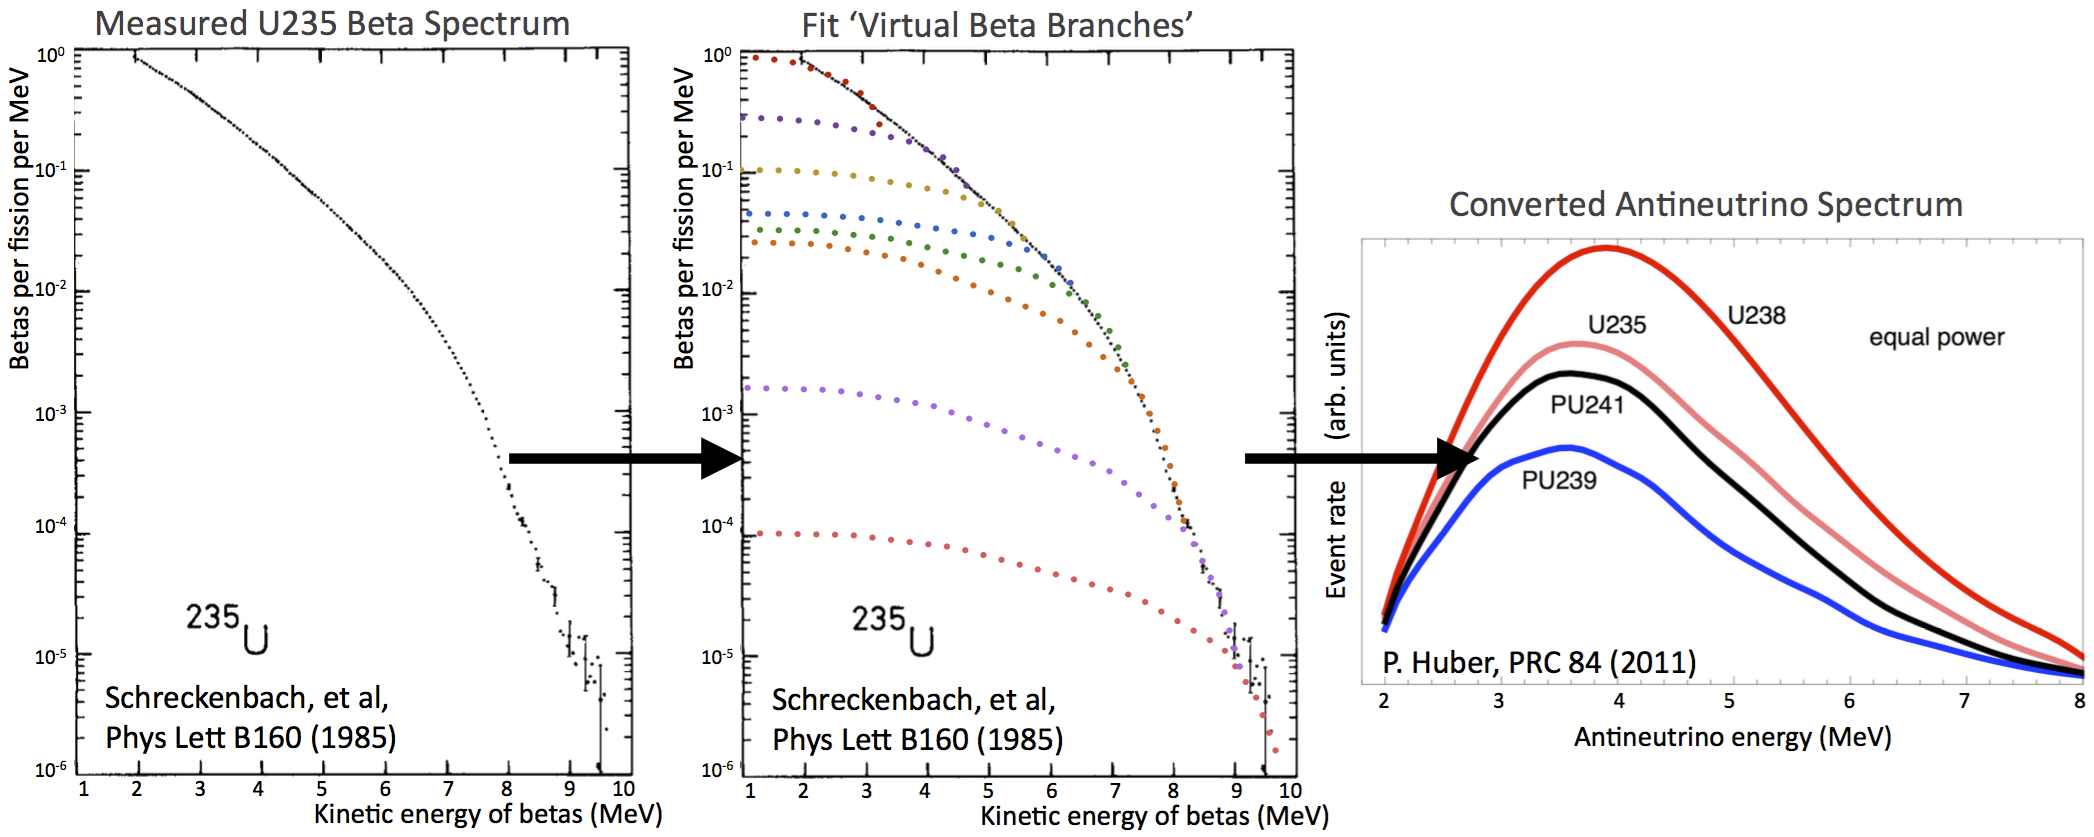
\includegraphics[width=0.7\linewidth]{tex/3-reactorneutrinos-images/betaspecconversion_fixed}
%	\caption{}
%	\label{fig:betaspecconversionfixed}
%\end{figure}

The electron spectra for $^{235}$U, $^{239}$Pu, and $^{241}$Pu were measured at the Institut
Laue-Langevin (ILL) reactor in Grenoble, France in the 1980s \cite{VonFeilitzsch:1982jw,Schreckenbach:1985ep,Hahn:1989zr}, while the spectrum of $^{238}$U was more recently (2014) measured at the neutron source FRMII in Garching, Germany \cite{Haag:2013raa}.
The ILL measurements, along with a prediction of the $^{238}$U $\bar{\nu_{e}}$ spectrum using the summation method by Vogel \cite{PhysRevC.24.1543}, became known as the ``ILL-Vogel" flux model and was the main model used until 2011.

In 2011 Mueller \textit{et al.} improved the prediction of the reactor antineutrino spectra by employing a method that combined information from the nuclear databases and the measured electron spectra from ILL \cite{Mueller}. 
This was followed by a further improvement by Huber who applied higher order corrections making use of the conversion method and minimizing the use of the databases as much as possible \cite{Huber}.

Though much work has been done to accurately model the reactor antineutrino spectra both methods are subject to uncertainties in the subdominant corrections to beta-decay. This includes radiative, weak magnetism, and finite size corrections along with uncertainties in the spectrum shape of forbidden transitions which are summarized in Ref.\cite{HayesVogel}. 
Besides the model uncertainties there are also experimental uncertainties that arise from knowing the thermal power of the reactor, its time-dependent fuel composition, and the fission energies of the dominant isotopes.
All of these uncertainties result in a 10-20\% relative uncertainty on the reactor antineutrino spectra using the \textit{ab initio} method and $\sim$5 \% uncertainty on the conversion approach \cite{Qian:2018wid}.



\section{Detection of Reactor Neutrinos}

Though there are several methods that can be used to detect reactor neutrinos, including charge-current ($\bar{\nu_e} + d \rightarrow n + n + e^+$), neutral-current ($\bar{\nu_e} + d \rightarrow n + p + \bar{\nu_e}$), and antineutrino-electron elastic scattering ($\bar{\nu_e} + e^- \rightarrow \bar{\nu_e} + e^-$), the one employed by most experiments is IBD ($\bar{\nu_e} + p \rightarrow e^+ + n$).
The IBD reaction energy threshold is 1.8 MeV and the cross section is relatively high, $\sim 63 \times 10^{-44} \textrm{cm}^2/\textrm{fisson}$ integrated over the entire reactor neutrino energy spectrum \cite{Qian:2018wid}, and can be written as
\begin{equation}
	\sigma^{(0)} \simeq 9.52 \times \left(\frac{E_e^{(0)}p_e^{(0)}}{\textrm{MeV}^2}\right) \times 10^{-44}\textrm{cm}^2
\end{equation}
where $E_e$ and $p_e$ are the energy and momentum of the final-state positron. 

An IBD event is selected by a pair of coincident signals consisting of a positron ionization and annihilation as the prompt signal and a time delayed neutron capture on a proton or nucleus as the delay signal. 
The neutrino energy can be backtracked from the prompt signal as
\begin{equation}	
	E_{\bar{\nu}} = E_{prompt} + 0.78~\textrm{MeV} + T_n
\end{equation}
where $T_n$ is the kinetic energy of the recoil neutron which is much smaller than the energy of the neutrino and can therefore be ignored in most cases. 
The IBD cross-section increases with energy, whereas the $\bar{\nu_{e}}$ spectrum decreases with energy creating a detected energy spectrum that peaks around 3.8 MeV and dies off after $\sim$8 MeV, as seen in Figure~\ref{fig:vogel-fig02}. 

In addition to great background rejection and good reconstruction of the neutrino energy, the IBD method of detecting neutrinos also allows the use of liquid scintillators and water as detection mediums. 

\begin{figure}[h]
	\centering
	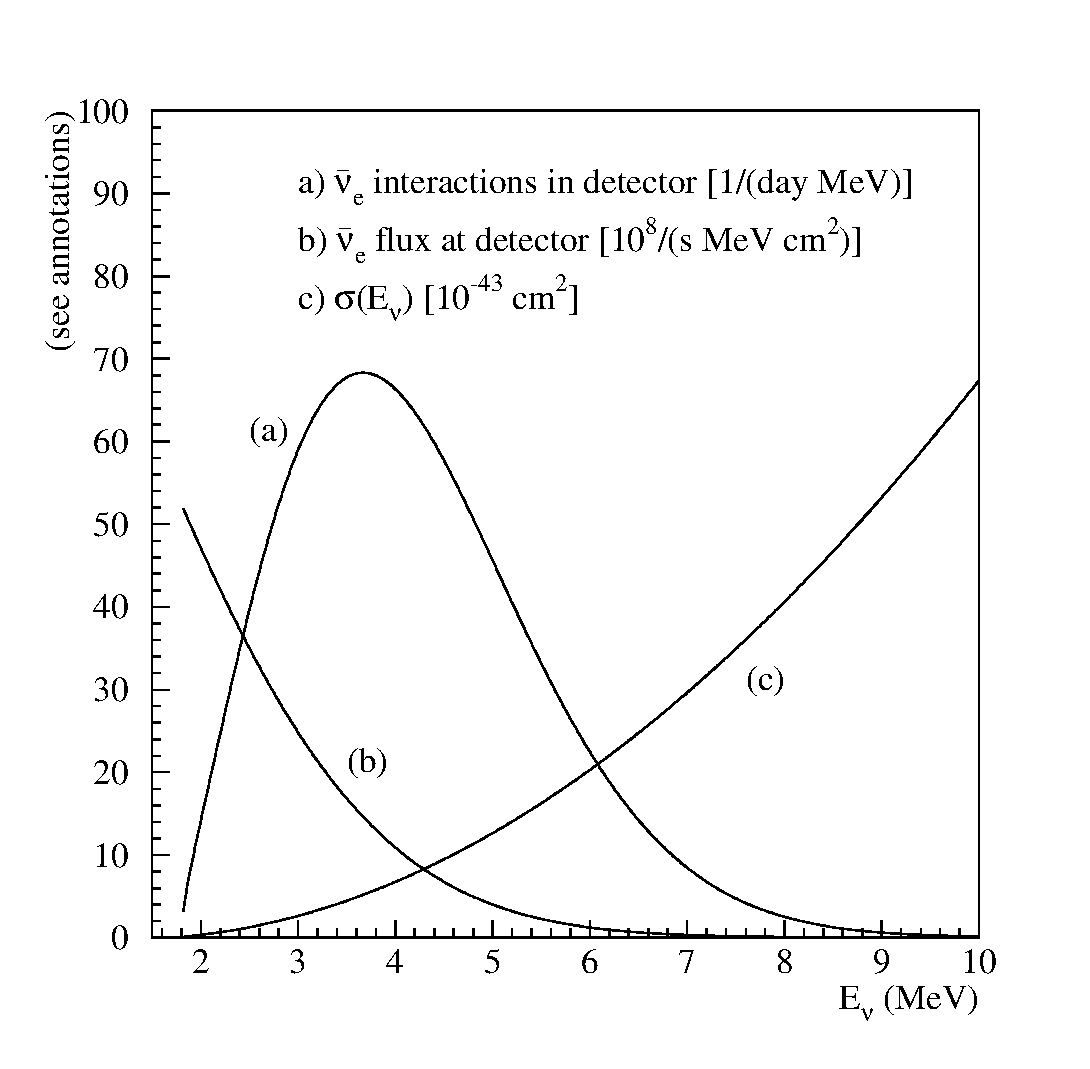
\includegraphics[width=0.55\linewidth]{tex/3-reactorneutrinos-images/vogel-fig02}
	\caption[The IBD spectrum.]{The IBD spectrum (curve (a)) measured by a 12-ton fiducial mass detector located 0.8 km from a 12-GW$_{th}$ power reactor along with the reactor flux (curve (b)) and IBD cross section (curve (c)) as a function of energy \cite{PDG}.}
	\label{fig:vogel-fig02}
\end{figure}


\section{The Reactor Antineutrino Anomaly}

Several experiments have, and continue to use reactor antineutrinos as a probe of neutrino oscillation. 
A reactor neutrino disappearance $P(\bar{\nu_{e}} \rightarrow \bar{\nu_{e}})$ experiment located at a distance L $\sim$ 1 km can measure $\sin^2\Delta_{31}$. At that baseline, the amplitude of the oscillation at the first maximum of $\sin^2\Delta_{31}$ is $\sin^22\theta_{13}$ (recall Eq.~\ref{eq:oscprob}), providing a direct measurement of $\theta_{13}$.
Three experiments were designed to make a measurement of this mixing angle, Daya Bay in China, RENO in Korea, and Double Chooz in France. 

The Daya Bay Reactor Neutrino Experiment was located at the Daya Bay nuclear reactor power plant in southern China that consists of six 2.9 GW$_{th}$ reactors. They employed two groups of near (512 m, 561 m) and one group of far (1,579 m) antineutrino detectors (AD) in order to suppress the reactor flux uncertainties \cite{An:2015qga,DayaBayAnomaly}.
The IBD yield measured for each AD is shown in Figure~\ref{fig:dayabayflux} and it can be seen that, after correcting for small variations of fission fractions among the different sites, all rates are consistent with each other. Though results between detectors agree, the disagreement between the experimental results and most recent model calculations (Huber+Mueller) is troubling. 

\begin{figure}[h]
	\centering
	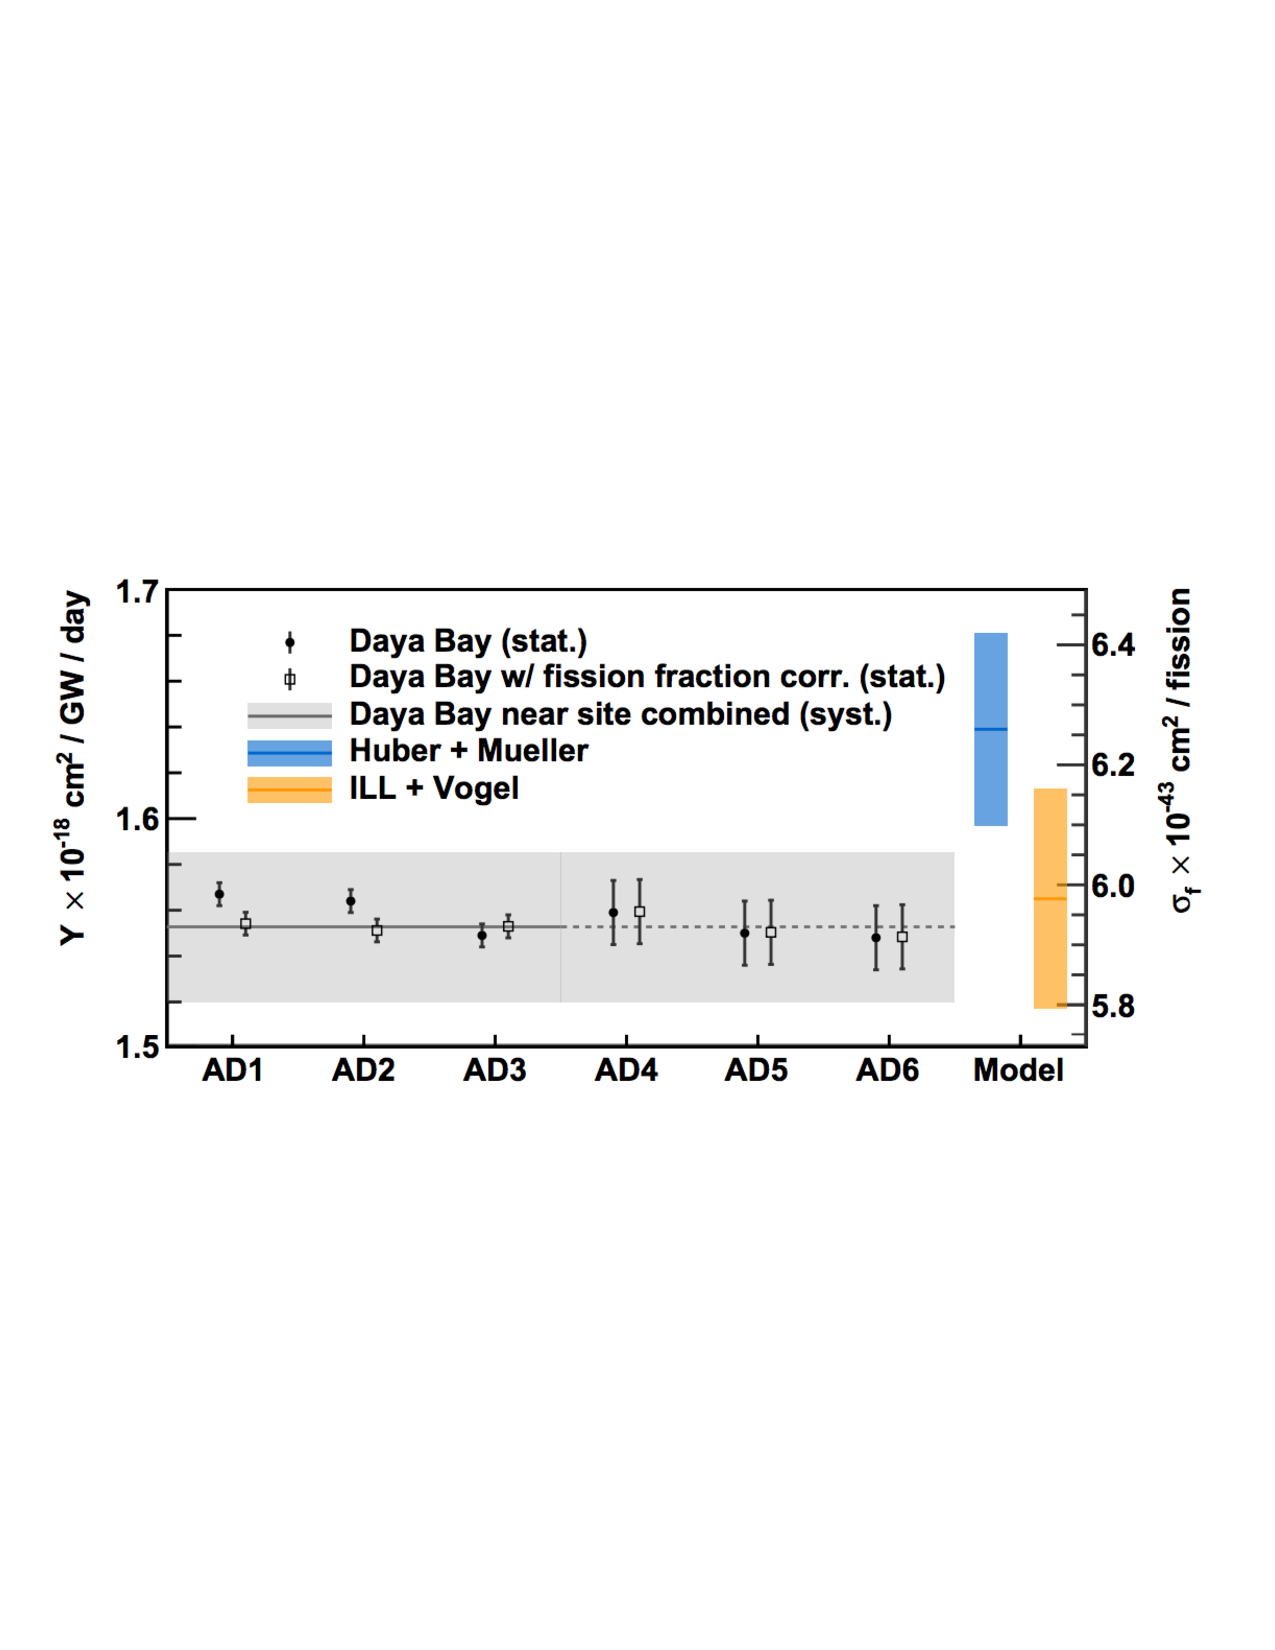
\includegraphics[width=0.7\linewidth]{tex/3-reactorneutrinos-images/DayaBayFlux}
	\caption[Daya Bay $\bar{\nu_{e}}$ flux.]{Rate of reactor antineutrino candidate events in Daya Bay's six detectors \cite{DayaBayAnomaly}. The average of the three near detectors is shown as the gray line, extended though the far detectors as a dotted gray line. Also shown are the rates predicted using the Huber+Mueller (blue) and ILL+Vogel (orange) models.}
	\label{fig:dayabayflux}
\end{figure}

In order to obtain a wider picture, the Daya Bay average IBD yield at the flux-weighted baseline (573 m) of the two near detector sites was compared to measurements from nineteen other short-baseline ($<$1000 m) experiments as shown in Figure~\ref{fig:worldavgflux}. 
The global average, including the most recent Daya Bay calculation, results in a ratio of measured to expected yield of 0.945 $\pm$ 0.007 (exp.) $\pm$ 0.023 (model) with respect to the Huber+Mueller model, a $\sim$6\% deficit \cite{DayaBayFlux2018}.
If the model uncertainty is to be trusted this ratio suggests reactor $\bar{\nu_{e}}$ disappearance as close as L$<$10 m, a phenomenon not covered in the standard 3-flavor neutrino mixing model \cite{HayesVogel}.  
This predicament has been labeled the ``reactor antineutrino anomaly" (RAA). 

\begin{figure}[H]
	\centering
	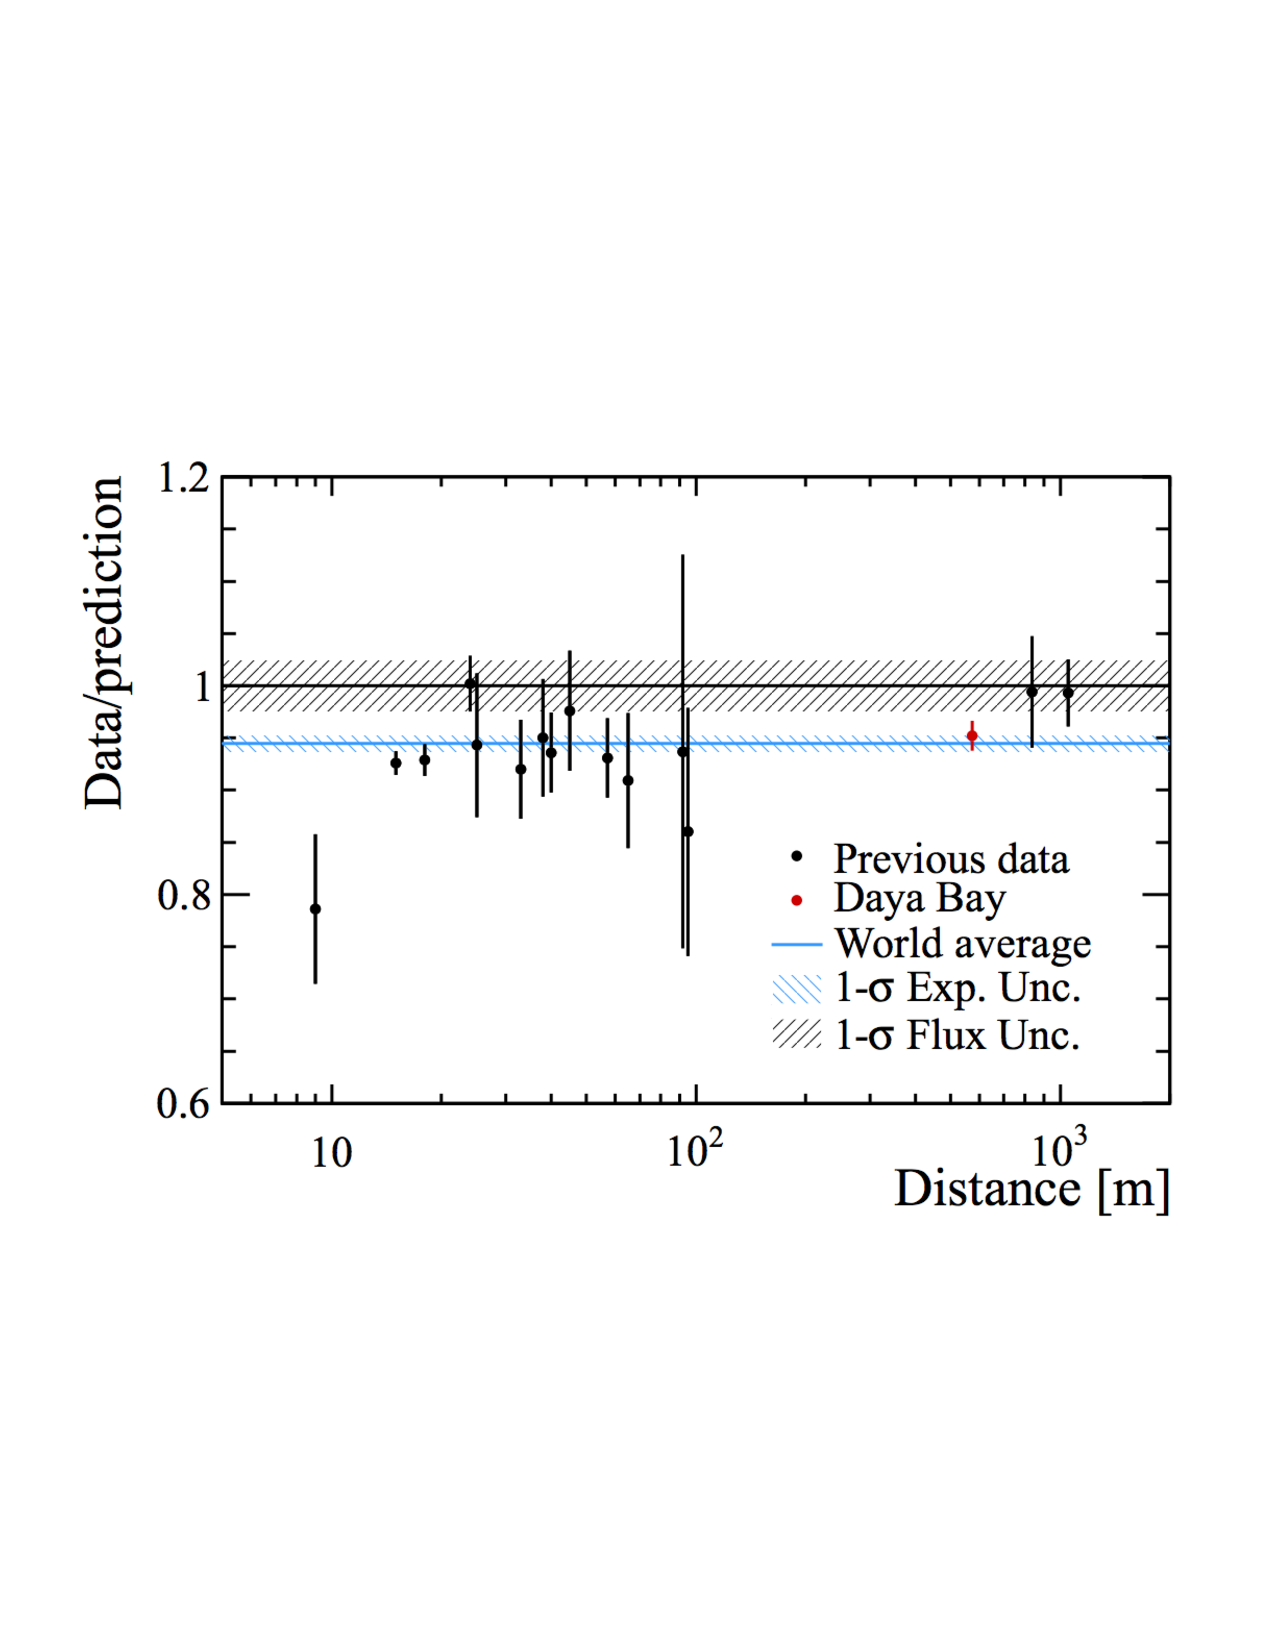
\includegraphics[width=0.6\linewidth]{tex/3-reactorneutrinos-images/WorldAvgFlux}
	\caption[World average of reactor $\bar{\nu_{e}}$ flux. ]{The measured reactor $\bar{\nu_{e}}$ rate, normalized to the Huber+Mueller model prediction, as a function of distance from the reactor \cite{DayaBayFlux2018}. The rate is corrected for 3-flavor neutrino oscillations at each baseline. The blue shaded region represents the global average and its 1$\sigma$ uncertainty. The 2.7$\sigma$ model uncertainty is shown as a band around unity.}
	\label{fig:worldavgflux}
\end{figure}

One hypothesis for explaining the reactor anomaly is that reactor neutrinos are oscillating into a new type of neutrino, a sterile neutrino. 
A sterile neutrino is a right-handed neutrino that does not take part in weak interactions except those induced by mixing with active neutrinos \cite{Abazajian:2012ys}. 
Evidence for sterile neutrinos has also been observed in non-reactor neutrino experiments. 
Specifically, the Liquid Scintillation Neutrino Detector (LSND)  measured an excess of $\bar{\nu_{e}}$ ($>$3$\sigma$) events \cite{Aguilar:2001ty} along with excesses measured by the Mini Booster Neutrino Experiment (MiniBooNE) of $\nu_{e}$ (3.4$\sigma$) and $\bar{\nu_{e}}$ (2.8$\sigma$) \cite{Aguilar-Arevalo:2013pmq}.
Two solar neutrino detectors, the Soviet–American Gallium Experiment (SAGE) and Gallium Experiment (GALLEX), have observed a deficit in electron neutrinos produced by intense artificial $^{51}$Cr and $^{37}$Ar radioactive sources at a significance of 3$\sigma$ \cite{Giunti:2010zu}.

All of these anomalies hint at short-baseline oscillations of electron neutrinos. 
The simplest way to explain these discrepancies is to add onto the standard model using the 3+1 oscillation model in which there are three active neutrinos and one sterile. This would introduce three new mixing angles, $\theta_{14}$ being the one of interest in reactor neutrino experiments.
A global fit of this model to neutrino data, including results from reactor experiments, SAGE and GALLEX, MiniBooNE, and spectrum measurements from ILL, result in oscillation constraints $\Delta m^2_{14} > 1.5 \textrm{eV}^2$ and $\sin^2(2\theta_{14}) = 0.14 \pm 0.08$, as shown in Figure~\ref{fig:raabestfitpoint} \cite{Mention:2011rk}.

\begin{figure}[t]
	\centering
	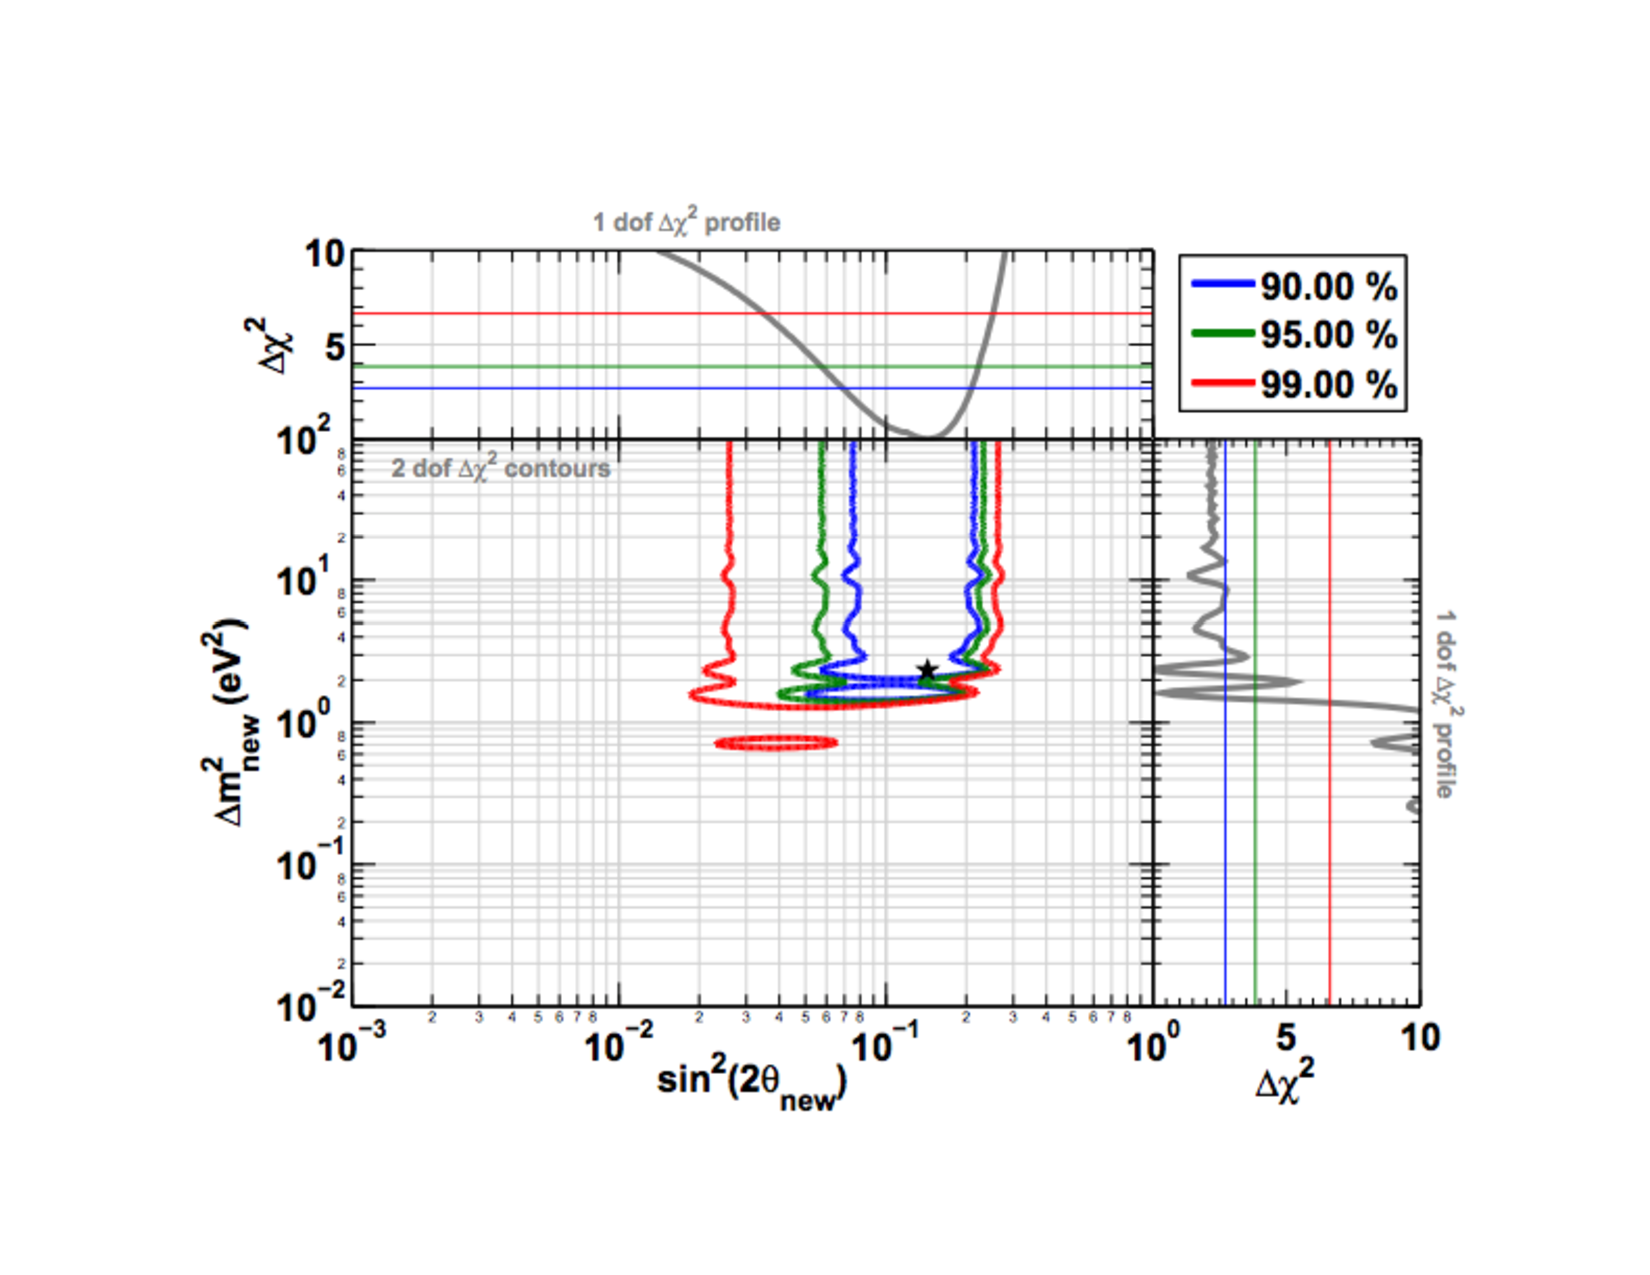
\includegraphics[width=0.7\linewidth]{tex/3-reactorneutrinos-images/RAA_BestFitPoint}
	\caption[]{Allowed regions in the $\sin^2(2\theta_{14})-\Delta m^2_{14}$ plane resulting from a fit of the 3+1 neutrino model to results from reactor neutrino experiments, SAGE and GALLEX, MiniBooNE, and spectrum measurements from ILL. This global fit results in the constraints $\Delta m^2_{14} > 1.5 \textrm{eV}^2$ and $\sin^2(2\theta_{14}) = 0.14 \pm 0.08$ \cite{Mention:2011rk}.}
	\label{fig:raabestfitpoint}
\end{figure}

An alternative explanation is that the flux predictions are incorrect and have larger uncertainties than those currently applied. 
The idea that the calculated reactor antineutrino flux is not well understood is bolstered by results from Daya Bay \cite{DayaBayAnomaly}, RENO \cite{Seo:2016uom}, and Double Chooz \cite{DoubleChooz:2019qbj} in which a ``bump" was observed in the experimentally measured antineutrino energy spectrum relative to the model spectrum, shown in Figure~\ref{fig:spectrums}.
Whether either or both hypothesis are true, and solve the reactor antineutrino anomaly, is a topic of great interest in the neutrino community and several experiments have been designed to address this matter.


\begin{figure}[t]
	\centering
	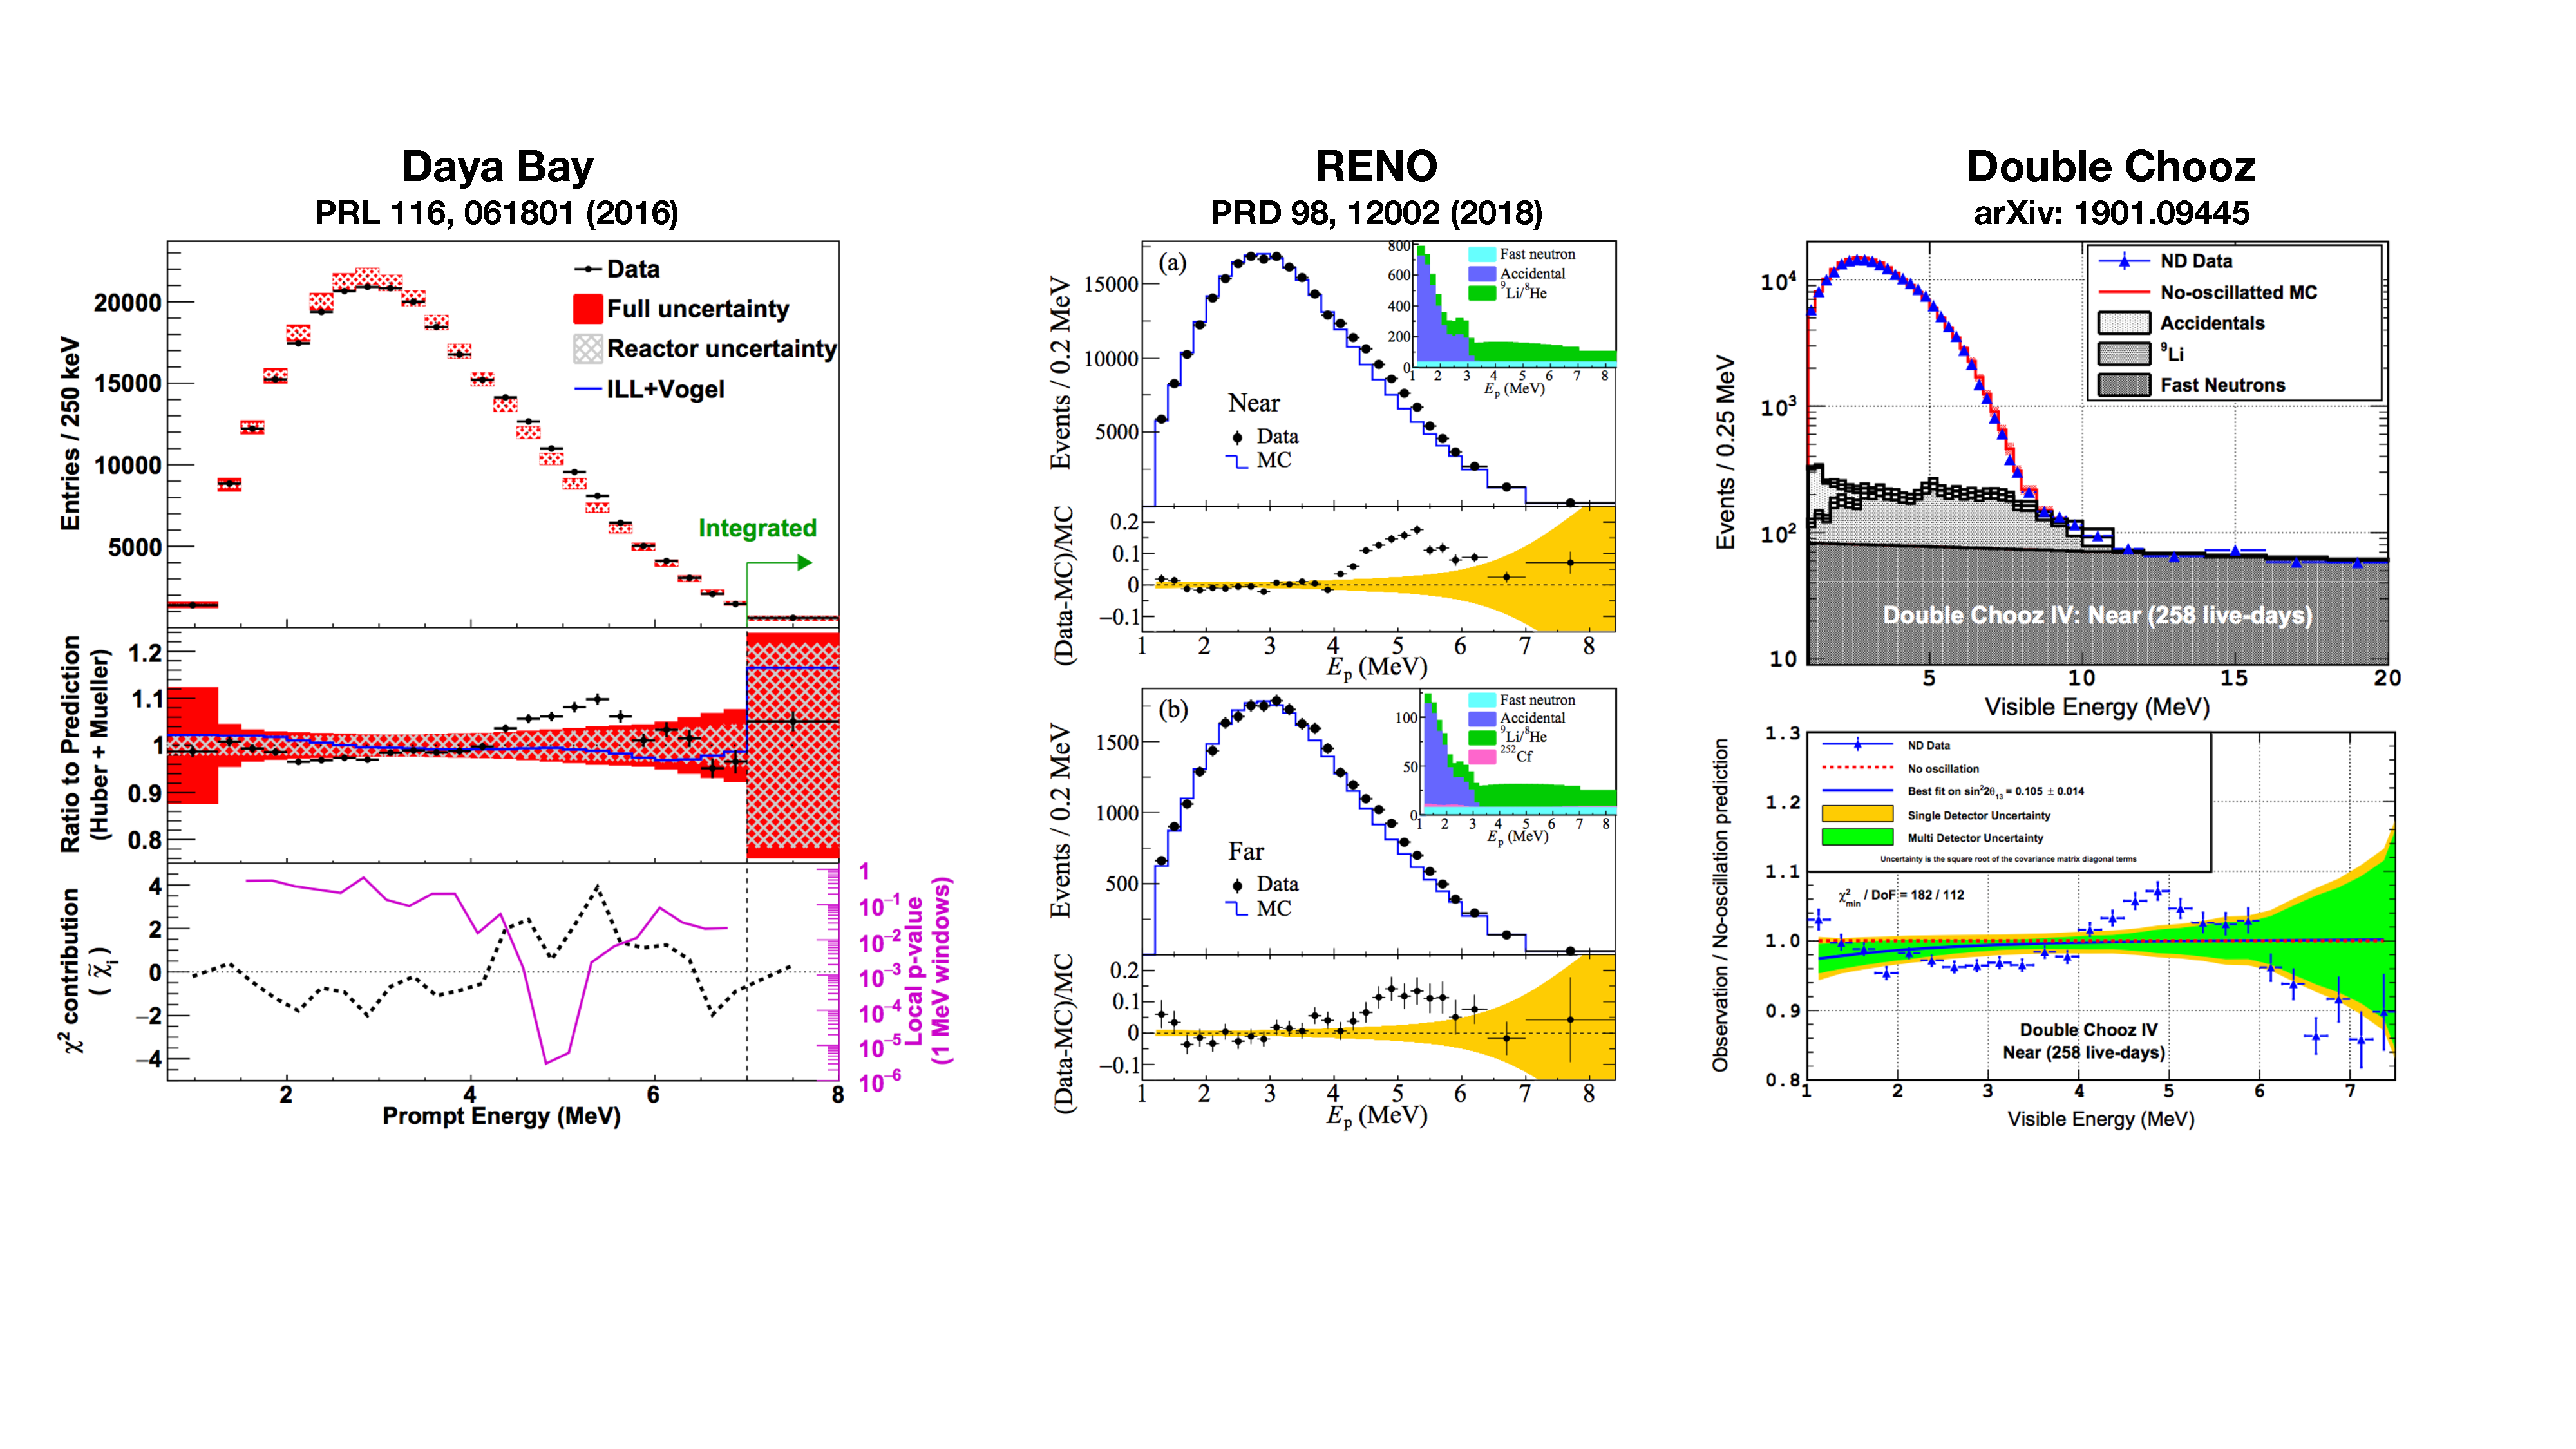
\includegraphics[width=1\linewidth]{tex/3-reactorneutrinos-images/Spectrums}
	\caption[Spectrums.]{A comparison between the predicted and measured prompt energy spectra of IBD events in Daya Bay \cite{DayaBayAnomaly}, RENO \cite{Seo:2016uom}, and Double Chooz \cite{DoubleChooz:2019qbj}. All experiments observe an excess of events above uncertainty in the model spectrum in the 4-6 MeV region.}
	\label{fig:spectrums}
\end{figure}


